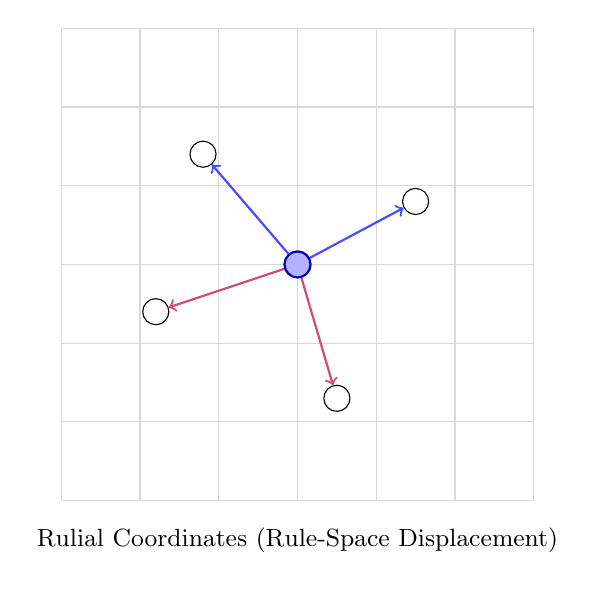
\begin{tikzpicture}[
    point/.style={circle, draw=black, fill=white, minimum size=6pt},
    active/.style={circle, draw=blue!70!black, fill=blue!30, minimum size=8pt, thick},
    vector/.style={->, thick},
    grid/.style={gray!30, thin}
]

% Grid
\foreach \i in {-3,-2,...,3}{
    \draw[grid] (\i,-3) -- (\i,3);
    \draw[grid] (-3,\i) -- (3,\i);
}

% Points
\node[active] (A) at (0,0) {};
\node[point] (B) at (1.5,0.8) {};
\node[point] (C) at (-1.2,1.4) {};
\node[point] (D) at (0.5,-1.7) {};
\node[point] (E) at (-1.8,-0.6) {};

% Vectors (showing rulial drift)
\draw[vector, blue!70] (A) -- (B);
\draw[vector, blue!70] (A) -- (C);
\draw[vector, purple!70] (A) -- (D);
\draw[vector, purple!70] (A) -- (E);

\node at (0,-3.5) {\small Rulial Coordinates (Rule-Space Displacement)};

\end{tikzpicture}